\documentclass[11pt]{article}

% ---------------------------------------------------------------------------
% Handout: reading _s2_closer.py — bracket matching, bounded Dyck, depth wall.
% Compile:  module load texlive/2025 && pdflatex closer_handout.tex   (run twice)
% All traced numbers verified by _trace_closer.py (== module == grammar_oracle).
% ---------------------------------------------------------------------------

\usepackage[margin=2.0cm]{geometry}
\usepackage{amsmath,amssymb}
\usepackage{xcolor}
\usepackage{tikz}
\usetikzlibrary{positioning,calc,arrows.meta,decorations.pathreplacing,fit,backgrounds}
\usepackage{forest}
\usepackage[most]{tcolorbox}
\usepackage{booktabs}
\usepackage{listings}
\usepackage{parskip}
\usepackage{microtype}

% --- palette ---------------------------------------------------------------
\definecolor{headc}{HTML}{1B7F3B}
\definecolor{compc}{HTML}{1F5FBF}
\definecolor{flipc}{HTML}{C0392B}
\definecolor{invc}{HTML}{555555}
\definecolor{panel}{HTML}{F4F1EA}
\definecolor{codebg}{HTML}{F7F7F4}

\newcommand{\head}[1]{\textcolor{headc}{#1}}
\newcommand{\comp}[1]{\textcolor{compc}{#1}}
\newcommand{\flip}[1]{\textcolor{flipc}{#1}}
\newcommand{\code}[1]{\texttt{#1}}

% --- callout boxes ---------------------------------------------------------
\newtcolorbox{rulebox}[1][]{colback=panel,colframe=black!70,boxrule=0.6pt,
  arc=2pt,left=6pt,right=6pt,top=4pt,bottom=4pt,title={#1},fonttitle=\bfseries}
\newtcolorbox{keybox}[1][]{colback=flipc!6,colframe=flipc!75,boxrule=0.8pt,
  arc=2pt,left=6pt,right=6pt,top=4pt,bottom=4pt,title={#1},fonttitle=\bfseries}

% --- python listing style --------------------------------------------------
\lstdefinestyle{py}{
  language=Python, basicstyle=\ttfamily\small, columns=fullflexible,
  keepspaces=true, showstringspaces=false, breaklines=true,
  backgroundcolor=\color{codebg}, frame=single, rulecolor=\color{black!25},
  framexleftmargin=3pt, xleftmargin=6pt, xrightmargin=4pt, aboveskip=6pt, belowskip=4pt,
  commentstyle=\color{invc}\itshape, keywordstyle=\color{compc}\bfseries,
  stringstyle=\color{headc}, emphstyle=\color{flipc}\bfseries,
  emph={kqv,select,sel_width,index_select,tok_map,where,indices,geq,equals},
}
\lstset{style=py}

% --- token-flow diagram helper (HI row over HF row with permutation arcs) ---
\newcommand{\tokflow}[4]{%
\begin{tikzpicture}[
   tok/.style={draw=black!55, fill=white, rounded corners=1.5pt,
               minimum height=6.5mm, inner xsep=3pt, font=\footnotesize},
   every node/.style={anchor=center}]
  \def\dx{#1}
  \foreach \i/\lab in {#2}{ \node[tok] (hi\i) at (\i*\dx,2.35) {\lab}; }
  \foreach \m/\lab in {#3}{ \node[tok] (hf\m) at (\m*\dx,0) {\lab}; }
  \node[font=\scriptsize\bfseries, text=invc] at (-1.05,2.35) {HI};
  \node[font=\scriptsize\bfseries, text=invc] at (-1.05,0)    {HF};
  \foreach \a/\b/\c/\t in {#4}{
     \draw[\c, line width=1.1pt, -{Stealth[length=4pt]}, opacity=0.9]
        (hi\a.south) to[out=-90,in=90] node[midway, sloped, above=-1pt,
        font=\tiny, text=\c]{\t} (hf\b.north);
  }
\end{tikzpicture}}

\begin{document}

\begin{center}
  {\LARGE\bfseries Reading \texttt{\_s2\_closer}}\\[3pt]
  {\large Recovering unmarked spans by bracket-matching --- and why that is bounded Dyck}\\[3pt]
  {\small \texttt{experiments/22\_rasp\_l\_hi\_hf/\_s2\_closer.py} \; (Strategy A, the chosen winner)}
\end{center}
\vspace{-2pt}\hrule\vspace{6pt}

\noindent This program turns a \emph{head-initial} sentence into its \emph{head-final} reordering
using only the length-generalizing transformer primitives of RASP-L (Weiss et al.\ 2021; Zhou et
al.\ 2024): elementwise maps, relative-position reads, and attention-based counting. The whole
task reduces to one hard sub-problem --- \textbf{recovering the constituent spans from a flat
string with no brackets} --- and \texttt{\_s2\_closer} solves it by explicitly finding, for each
clause opener, where its clause \emph{closes}. That is bracket-matching, and its cost in layers is
exactly the story of \textbf{bounded Dyck} languages.

% ==========================================================================
\section{The pipeline and where \texttt{closer} sits}

HF is a \emph{permutation} of HI: every token keeps its identity and only moves. So the program
never ``generates'' --- it computes, per HI position $i$, a target slot and gathers:
\[
  \text{hf\_pos}(i) = i + \text{disp}(i),\quad
  \text{disp}(i)=\!\!\sum_{\substack{F\ \flip{\text{flip}},\ i\in F}}\!\!
  \big(\head{+|\text{comp}(F)|}\ (i\in\head{\text{head}}),\ \comp{-|\text{head}(F)|}\ (i\in\comp{\text{comp}})\big).
\]
Three stages:

\begin{center}\footnotesize
\begin{tabular}{@{}llll@{}}
\toprule
 & stage & what & primitives\\
\midrule
1 & \textbf{local POS + role} & word $\to$ lexical class $\to$ fine POS \& verb role & \code{tok\_map} + relative reads\\
2 & \textbf{spans (\flip{closer})} & recover clause/phrase \emph{end} of every opener, then \code{depth} \& \code{disp} & relaxation + \emph{stabbing} counts\\
3 & \textbf{gather} & invert the permutation, place tokens & two \code{kqv} heads\\
\bottomrule
\end{tabular}
\end{center}

\noindent Stages 1 and 3 are easy and provably length-generalizing (Stage 3 was verified $2000/2000$
when fed the oracle's \code{disp}, independent of Stage 2). \textbf{Everything hard is Stage 2},
and \texttt{\_s2\_closer} is one of four independent constructions of it. This handout reads that
construction end-to-end.

% ==========================================================================
\section{Why spans are the hard part: unmarked, coincident closes}

To know which flip nodes enclose token $i$ --- and how big their complements are --- we need each
constituent's \textbf{span} $[q,\,e(q)]$. In a bracketed string that is trivial. Here it is not:

\begin{keybox}[Two facts that make this genuine bracket-matching]
\textbf{(1) Closes are unmarked.} The surface string has openers you can \emph{see} (a \code{that}
begins a clause) but \emph{no} close symbol --- a clause just ends where its verb phrase ends, which
you must \emph{infer} from parts of speech.\\[3pt]
\textbf{(2) Closes can coincide (multiplicity $>1$).} A \code{CP\_sent} sitting at the right edge of
a relative clause closes \emph{together} with it: in \emph{the cat [that claims [that the dog
swims]] runs}, both clauses end right after \emph{swims}.
\end{keybox}

\noindent So Stage 2 must \emph{compute} the matching close $e(q)$ for every opener $q$. The
recursion is real: a clause's end depends on its complement's end, which for an embedded clause is
\emph{another} clause's end. Once $e(q)$ is known, the nesting depth is a count:
\[
  \boxed{\ \text{depth}(i) \;=\; \#\{\,\text{openers } q \le i \ :\ e(q) \ge i\,\}\ }
  \qquad\text{(how many opener--close intervals ``stab'' position $i$).}
\]

% ==========================================================================
\section{Stage 1: lexical class and verb role (all local)}

A fixed word$\to$class embedding, then four relative-position reads to see the neighbours, then a
few elementwise decisions. No cross-clause information yet.

\begin{lstlisting}
lc      = tok_map(hi_ids, _lexclass)         # D, N_sing, N_prop, Adj, Adv, THAT, V, OTHER
prev_lc = _read_off(lc, -1); next_lc = _read_off(lc, +1)   # lc[i-1], lc[i+1] (rel. reads)
is_crel = isthat & (prev_lc == NSING)        # 'that' after a common noun -> relative C_rel
nn_lc   = where(next_lc == ADV, next2_lc, next_lc)         # next NON-adverb class
role    = where(nn_lc == THAT, 3,            # V_cp   (takes a clause)      role 3
          where((nn_lc==D)|(nn_lc==NPROP), 2,# V_dp   (takes an object DP)  role 2
          where(is_intr, 1, 4)))             # intransitive 1 / object-gap 4
\end{lstlisting}

\noindent \textbf{Verb role} is the key local disambiguation: a verb's role decides whether it heads
a \flip{flip} \code{VP} and what its complement is. Roles: \code{1}=intransitive, \code{2}=takes an
object DP, \code{3}=takes a clause, \code{4}=object-gap (a transitive verb whose object was
relativized away, e.g.\ \emph{that the boy chases}). Roles 2 and 3 are the VP-flip heads; 1 and 4
never flip. All of Stage 1 is content + relative offset $\Rightarrow$ length-generalizing.

% ==========================================================================
\section{Stage 2a: the \flip{closer} --- END pointers by relaxation}

The core. We maintain four \textbf{end pointers}, one per constituent type, initialised to
``ends at itself'' and then refined by a fixed number \code{K} of \emph{relaxation sweeps}:

\begin{center}\footnotesize
\begin{tabular}{@{}ll@{}}
\toprule
pointer & meaning: last index of the \dots starting here\\
\midrule
\code{dpfull} & DP (\emph{including} any relative clause hanging off its noun)\\
\code{vpe}    & VP (verb $+$ its complement: object DP, or embedded CP, or nothing)\\
\code{rce}    & \code{CP\_rel} (a relative clause \code{that \dots})\\
\code{cpe}    & \code{CP\_sent} (a sentential clause \code{that \dots})\\
\bottomrule
\end{tabular}
\end{center}

\begin{lstlisting}
dpfull, vpe, rce, cpe = dp_end_flat, hb_end, idx, idx  # init: each "ends at itself"
for _ in range(K):                     # each sweep resolves ONE more nesting level
    dpfull = where(dp_has_rc, rce_at_rc, dp_end_flat)   # DP skips its rel. clause
    vpe = where(role in {1,4}, hb_end,          # intrans/objgap: stop at the verb
           where(role==2, dpfull_at_hb1,        # +object DP: end of that object
           where(role==3, cpe_at_hb1, idx)))    # +clause: end of the that-CP
    rce = where(is_crel, subj?vpe_at_q1:dpfull_at_q1+1, idx)   # CP_rel end
    cpe = where(is_c, vpe_at_vpos, idx)         # CP_sent: its inner VP's end
e = where(is_crel, rce, where(is_c, cpe, idx))  # clause end e(q) per 'that'
\end{lstlisting}

\begin{rulebox}[Why a \emph{sweep} is one attention hop]
Each assignment reads a pointer \emph{at another position} (\code{index\_select}, one attention
head): e.g.\ a clausal verb's \code{vpe} copies the \code{cpe} of the \code{that} just after it;
that \code{cpe} in turn copied the \code{vpe} of \emph{its} inner verb. A single sweep can only
follow \textbf{one} such link. To resolve a clause whose complement is a clause whose complement
is a clause, you must run the sweep once per level: \textbf{sweeps needed $=$ nesting depth}. This
is the load-bearing fact for everything in \S8.
\end{rulebox}

% ==========================================================================
\section{Stage 2b: depth and displacement as \emph{stabbing sums}}

With $e(q)$ known, \code{depth} is a single counting head --- count opener intervals that cover $i$:

\begin{lstlisting}
end_that = where(isthat, e, -1)             # only 'that' positions carry a real interval end
depth    = sel_width(select(end_that, indices, geq, causal=True))   # #{q<=i : e(q) >= i}
\end{lstlisting}

\noindent The \emph{same} stabbing trick expresses the whole displacement. Grouping the per-flip sum
by \textbf{flip type} gives four additive pieces, each a (weighted) count of enclosing flips of that
type plus a local head bonus:

\begin{center}\footnotesize
\begin{tabular}{@{}lll@{}}
\toprule
piece & flip type & how it is computed\\
\midrule
\code{d\_adv}   & \code{VP\_x\_adv} (verb$\leftrightarrow$adverb) & purely local: verb $+1$ if adverb follows, adverb $-1$\\
\code{d\_cp}    & \code{CP\_sent} $+$ \code{CP\_rel}              & $-\text{depth}$ everywhere; each \code{that} also $+|$its clause$|$\\
\code{d\_nprel} & \code{NP\_singular}$\to$[core, \code{CP\_rel}]  & core noun $+|$RC$|$; RC tokens $-|$core$|$ per enclosing RC (stab)\\
\code{d\_vp}    & transitive/clausal \code{VP}                   & head-block $+|$comp$|$; comp tokens $-|$head$|$ per enclosing VP (stab)\\
\bottomrule
\end{tabular}
\end{center}

\begin{keybox}[The one subtlety in reading these pieces]
Each of \code{d\_cp}, \code{d\_nprel}, \code{d\_vp} is a \textbf{stabbing sum}: a token pays into
\emph{every} enclosing flip of that type, not just its parent. That is why, below, \emph{likes}
gets $\code{d\_vp}=+1$: it is the \head{head} of its own object-taking VP ($+2$) \emph{and} sits
inside the outer clause-taking VP's complement ($-1$). Same additive rule as the tree formula in
\S1, just bucketed by flip type. All four sum to the oracle's \code{disp} (verified, and still exact
at depth 3 --- it is a tree identity, not a depth-2 coincidence).
\end{keybox}

\noindent \textbf{Stage 3} then inverts the permutation and gathers (two heads):
\begin{lstlisting}
hf_pos = idx + (d_adv + d_cp + d_nprel + d_vp)
src    = kqv(hf_pos, idx, idx, equals, causal=False)   # slot j <- the i with hf_pos[i]==j
out    = index_select(hi_ids, src, causal=False)       # place each HI token into its slot
\end{lstlisting}

% ==========================================================================
\section{Worked example (depth 1), every number verified}

\emph{John knows that Mary likes the dog} $\;\rightarrow\;$ \emph{John Mary the dog likes that knows}.
One opener, \code{that} at position~2, closing at $e=6$ (the clause \emph{that Mary likes the dog}
ends on \emph{dog}). Roles: \emph{knows}$=$clausal (3), \emph{likes}$=$transitive (2).

\begin{center}\small
\begin{tabular}{@{}rl ccc rrrr r@{}}
\toprule
$i$ & tok & role & $e(q)$ & depth & \code{d\_adv} & \code{d\_cp} & \code{d\_nprel} & \code{d\_vp} & disp\\
\midrule
0 & John  & --    & --  & 0 & $0$ & $0$  & $0$ & $0$  & $0$\\
1 & knows & cp    & --  & 0 & $0$ & $0$  & $0$ & $+5$ & $+5$\\
2 & that  & --    & $6$ & 1 & $0$ & $+4$ & $0$ & $-1$ & $+3$\\
3 & Mary  & --    & --  & 1 & $0$ & $-1$ & $0$ & $-1$ & $-2$\\
4 & likes & trans & --  & 1 & $0$ & $-1$ & $0$ & $+1$ & $0$\\
5 & the   & --    & --  & 1 & $0$ & $-1$ & $0$ & $-2$ & $-3$\\
6 & dog   & --    & --  & 1 & $0$ & $-1$ & $0$ & $-2$ & $-3$\\
\bottomrule
\end{tabular}
\end{center}

\begin{center}
\tokflow{1.75}
  {0/John, 1/knows, 2/that, 3/Mary, 4/likes, 5/the, 6/dog}
  {0/John, 1/Mary, 2/the, 3/dog, 4/likes, 5/that, 6/knows}
  {0/0/invc/0, 1/6/headc/{+5}, 2/5/headc/{+3}, 3/1/compc/{-2}, 4/4/invc/0, 5/2/compc/{-3}, 6/3/compc/{-3}}
\end{center}

\noindent Read \code{d\_cp}: everyone in the clause body gets $-\text{depth}=-1$; the \code{that}
additionally gets $+|$clause$|-\text{(outer CPs)} = +4$, i.e.\ it is the clause's head jumping over
its 4-token body. \code{d\_vp}: \emph{knows} is a clausal VP head over a 5-token complement ($+5$);
\emph{likes} nets $+1$ (its own $+2$ minus the outer VP's $-1$).

% ==========================================================================
\section{The relaxation in motion (depth 2) --- seeing the hop}

\emph{John knows that Mary knows that the dog swims}: two openers, \code{that}@2 (depth-1) and
\code{that}@5 (depth-2). \textbf{Both clauses close on \emph{swims} (position 8)} --- a
multiplicity-2 close. Here is $e(q)$ after each sweep (only the two \code{that} columns matter):

\begin{center}\small
\begin{tabular}{@{}l cccccccccc@{}}
\toprule
position $i$        & 0 & 1 & \textbf{2} & 3 & 4 & \textbf{5} & 6 & 7 & 8 \\
token               & John & knows & \textbf{that} & Mary & knows & \textbf{that} & the & dog & swims\\
\midrule
after \textbf{sweep 1} & . & . & \flip{$5$} & . & . & $8$ & . & . & . \\
after \textbf{sweep 2} & . & . & \head{$8$} & . & . & $8$ & . & . & . \\
final depth$(i)$    & 0 & 0 & 1 & 1 & 1 & 2 & 2 & 2 & 2 \\
\bottomrule
\end{tabular}
\end{center}

\noindent The \emph{inner} opener resolves to $e=8$ in \textbf{one} sweep (its complement
\emph{the dog swims} bottoms out immediately). The \emph{outer} opener cannot: after sweep~1 it
still thinks it closes at \flip{$5$} (it has only followed one link, to the inner verb), and only
after sweep~2 does it inherit the inner clause's true end and correct to \head{$8$}. \textbf{Depth~2
needed $\ge 2$ sweeps.} The Dyck-depth profile (bottom row) is exactly a bracket-nesting count:

\begin{center}
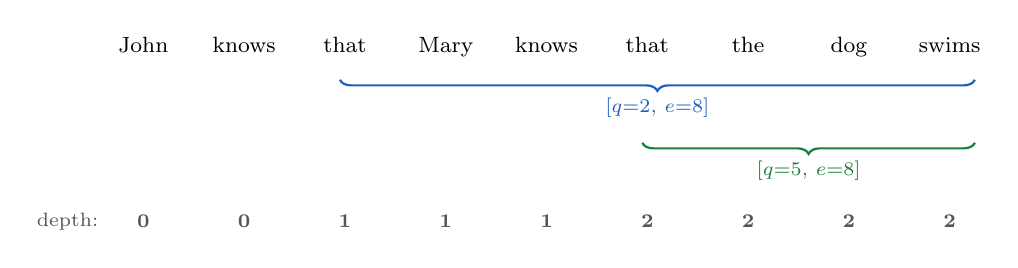
\begin{tikzpicture}[font=\footnotesize, xscale=1.28]
  \foreach \i/\w in {0/John,1/knows,2/that,3/Mary,4/knows,5/that,6/the,7/dog,8/swims}
     \node[anchor=base] at (\i,0) {\w};
  % interval brackets
  \draw[compc, thick, decorate, decoration={brace, amplitude=4pt, mirror}]
     (1.95,-0.35) -- node[below=3pt, font=\scriptsize, text=compc]{$[q{=}2,\,e{=}8]$} (8.25,-0.35);
  \draw[headc, thick, decorate, decoration={brace, amplitude=4pt, mirror}]
     (4.95,-1.15) -- node[below=3pt, font=\scriptsize, text=headc]{$[q{=}5,\,e{=}8]$} (8.25,-1.15);
  % depth profile
  \foreach \i/\d in {0/0,1/0,2/1,3/1,4/1,5/2,6/2,7/2,8/2}
     \node[font=\scriptsize\bfseries, text=invc] at (\i,-2.15) {\d};
  \node[font=\scriptsize, text=invc, anchor=east] at (-0.35,-2.15) {depth:};
\end{tikzpicture}
\end{center}

% ==========================================================================
\section{Relationship to Dyck-$(k,D)$}

\begin{rulebox}[Dyck-$k$ and Dyck-$(k,D)$]
\textbf{Dyck-$k$} is the language of balanced strings over $k$ kinds of bracket pairs; its defining
operation is the \emph{matching function} sending each opener to its unique closer. \textbf{Dyck-$(k,D)$}
adds a cap: nesting depth $\le D$ (Yao et al.\ 2021). Bounded depth is what separates
``recognizable by a fixed transformer'' from ``not''.
\end{rulebox}

\noindent \texttt{\_s2\_closer} is, at its heart, a Dyck-$(k,D)$ \emph{matcher}, with three twists
that make it harder than textbook Dyck:

\begin{center}\footnotesize
\begin{tabular}{@{}lll@{}}
\toprule
Dyck notion & in \texttt{\_s2\_closer} & twist\\
\midrule
opener      & a \code{that} token (visible)                    & --- \\
closer      & the clause end $e(q)$                            & \textbf{unmarked}: inferred from POS, not a symbol\\
matching $q\!\to\!e(q)$ & the relaxation loop               & mutually-recursive over DP/VP/CP types\\
depth $D$   & CP-nesting bound ($=2$ in the dataset)           & the \code{ROUNDS} knob is the machine's depth budget\\
$k$ types   & \code{CP\_sent} vs \code{CP\_rel} ($+$ DP/VP ends) & several typed brackets matched \emph{simultaneously}\\
coincident closes & multiplicity-2 ends                        & one position closes two brackets at once\\
\bottomrule
\end{tabular}
\end{center}

\noindent Strip the twists and you have the pure task ``for each open bracket, output the index of
its matching close, given depth $\le D$.'' The relaxation is precisely the standard bounded-Dyck
matching algorithm: propagate matches inward-to-outward, one nesting level per layer. The
constituent grammar dresses it up (unmarked, typed, coincident closes), but the \emph{cost
structure} --- layers proportional to $D$ --- is inherited unchanged from Dyck-$(k,D)$.

% ==========================================================================
\section{Theory implications}

\subsection{The demonstrated law: layers $=$ depth $+1$}
\texttt{ROUNDS} is a fixed block of transformer layers. Sweeping it reproduces a sharp wall ---
re-verified directly: \code{ROUNDS=4} solves depth 3 ($40/40$), while \code{ROUNDS=3} fails it
entirely ($0/40$):
\[
  R \text{ rounds resolve CP-depth} \le R-1; \qquad \text{depth } R \text{ fails entirely.}
\]
Because a clause's end depends on its complement's end (another clause, for \code{V\_cp}), the
END-pointer dependency chain is as long as the nesting is deep; one sweep extends every pointer by
one level, so resolving depth $d$ needs $\Omega(d)$ \emph{sequential} sweeps $=\Omega(d)$ layers.
A \textbf{fixed}-depth transformer therefore represents HI$\to$HF only up to some depth and cannot
extend to deeper inputs --- \textbf{no amount of data helps}, because deeper inputs need more
sequential composition than the architecture physically has.

\subsection{Length generalization $\ne$ depth generalization}
This is the crucial distinction. \emph{At a fixed depth}, every op in the program is content-based,
relative-position, or counting --- the RASP-L primitives that \textbf{do} length-generalize (Zhou
et al.\ 2024): a depth-2 sentence that is merely \emph{longer} is handled fine. What does
\emph{not} generalize is \textbf{depth}: the only programs for the matching function use
unbounded-depth bracket-matching, which lives outside the length-generalizing primitive set. So
structured reversal joins copy / reverse / unbounded-Dyck as a task that ``does not
length-generalize without a hint,'' and the \code{ROUNDS} knob makes the boundary explicit and
testable.

\subsection{Where this sits in expressivity theory}
\begin{itemize}\setlength{\itemsep}{1pt}
\item \textbf{Bounded Dyck is doable, at a price.} Transformers \emph{can} recognize Dyck-$(k,D)$,
  but the required depth grows with $D$ (Yao et al.\ 2021). Our linear \code{layers}$=$\code{depth}$+1$
  is a concrete, mechanism-level instance of that theorem.
\item \textbf{Unbounded Dyck is out of reach.} Fixed-depth (log-precision) transformers sit in a
  shallow, uniform-$\mathrm{TC}^0$-style circuit class (Merrill \& Sabharwal 2023); an unbounded
  stack for arbitrary nesting is outside it, and hard-attention cannot do unbounded Dyck or PARITY
  at all (Hahn 2020). Depth generalization to \emph{arbitrary} nesting is thus a hard
  \emph{expressivity} barrier, not a mere optimization one.
\end{itemize}

\subsection{Falsifiable predictions for the training splits}
\begin{keybox}[Two axes that must behave oppositely]
\textbf{Depth held out} (train depth $\le 1$, test depth $2$): the model is never forced to
\emph{use} the second sweep, so at depth 2 it hits the wall $\Rightarrow$ \textbf{predict failure}
(matches the empirical negatives in exps 10/16).\\[3pt]
\textbf{Object-gap $\to$ subject-gap relatives} (same depth): both gap types are the \emph{same}
\code{CP\_rel} flip and need \emph{no} extra nesting --- the gap only changes what sits \emph{inside}
the clause $\Rightarrow$ \textbf{predict transfer succeeds}. A failure here would be optimization,
not expressivity.
\end{keybox}

\subsection{Escape hatches (both consistent with the theory)}
\textbf{(a) Give depth as an input hint} --- index/scratchpad tricks (Zhou et al.\ 2024) so the model
\emph{reads} nesting instead of \emph{deriving} it; this literally provides the non-length-generalizing
part. \textbf{(b) Let layers scale with input} --- universal / looped transformers restore the
$\Omega(\text{depth})$ sequential budget, and depth generalization is back on the table. A plain
fixed-depth decoder trained on shallow data gets neither, so the wall stands.

% ==========================================================================
\section{Why the wall is intrinsic, not a quirk of this code}
The same $\Omega(\text{depth})$ wall appears in three independent Stage-2 constructions ---
\texttt{closer} (relaxation), \texttt{interval} (that/verb balance $+$ pointer-jumps),
\texttt{twolevel} (four families $+$ fix-point) --- each verified $100\%$ at depth $\le 2$ and each
failing one level past its round budget. A fourth (\texttt{gaplca}, pairwise flip-LCA) already
breaks at depth~3. Three different algorithms hitting the \emph{same} wall is the signature of a
property of the \emph{task}, not of a particular program: HI$\to$HF requires bounded-depth bracket
matching, and its layer cost is set by the depth $D$, exactly as Dyck-$(k,D)$ theory predicts.

\vfill
\begin{center}\footnotesize\itshape
Every traced value (roles, $e(q)$ per sweep, \code{depth}, the four \code{disp} pieces, HF) was
produced by \texttt{\_trace\_closer.py}, which reproduces \texttt{\_s2\_closer.hi\_to\_hf} verbatim
and asserts agreement with it and with \texttt{grammar\_oracle.py}.\\[2pt]
References: Weiss, Goldberg \& Yahav 2021 (RASP); Zhou et al.\ 2024 (RASP-L / length generalization);
Yao et al.\ 2021 (bounded hierarchical languages); Hahn 2020 (self-attention limits);
Merrill \& Sabharwal 2023 (log-precision transformers $\subseteq \mathrm{TC}^0$).
\end{center}

\end{document}
